\newenvironment{gtpartn}[1]{}{}
%% ============================================================ 41  NJC 2024 Promo Q4(b)
\defQ{41}{}{%
A curve with equation $y=\mathrm{h}(x)$ undergoes the following sequence of transformations.
\begin{center}\begin{tabular}{l}
\textbf{A}: A translation of 2 units in the positive direction of the $x$-axis.\\
\textbf{B}: A scaling parallel to the $x$-axis by factor of 3.\\
\textbf{C}: A reflection in the $y$-axis.
\end{tabular}\end{center}
The resultant curve has equation $y=-\dfrac{x^{2}}{6x+45}$. Find $\mathrm{h}(x)$. \mk{3}
\src{NJC 2024 Promo Q4(b)}}
\defS{41}{%
\begin{gtpart}{(b)}{3}\begin{topalign}
y&=-\frac{x^{2}}{6x+45}\\
&\text{C}^{-1}\text{: reflection in the $y$-axis }(x\to-x)\\
y&=-\frac{(-x)^{2}}{6(-x)+45}=-\frac{x^{2}}{-6x+45}\\
&\text{B}^{-1}\text{: scaling parallel to the $x$-axis by factor $\tfrac13$ }(x\to3x)\\
y&=-\frac{(3x)^{2}}{-6(3x)+45}=-\frac{9x^{2}}{-18x+45}=-\frac{x^{2}}{-2x+5}\\
&\text{A}^{-1}\text{: translation of 2 units in the negative $x$-direction }(x\to x+2)\\
y&=-\frac{(x+2)^{2}}{-2(x+2)+5}=-\frac{(x+2)^{2}}{-2x+1}\\
\mathrm{h}(x)&=\frac{(x+2)^{2}}{2x-1}
\end{topalign}\end{gtpart}}
%% ============================================================ 42  EJC 2025 Prelim P1 Q4
\defQ{42}{}{%
The diagram below shows the graph of $y=\mathrm{f}(2x)$. The graph has a turning point at $(2,0)$, and asymptotes with equations $x=0$ and $y=k$.
\begin{center}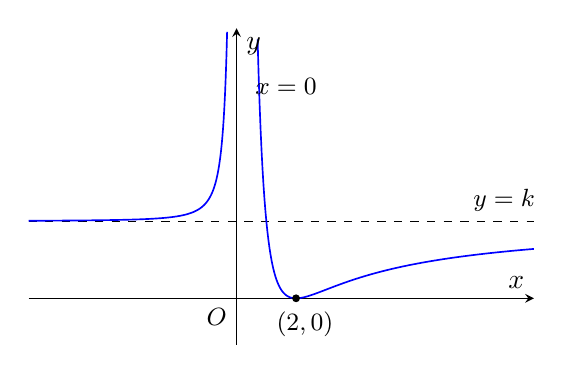
\begin{tikzpicture}
\begin{axis}[width=8cm,height=5.6cm,axis lines=middle,xmin=-7,xmax=10,ymin=-1.2,ymax=7,ticks=none,clip=false,restrict y to domain=-1.2:7,unbounded coords=jump,xlabel=$x$,ylabel=$y$]
\addplot[black,dashed,domain=-7:10]{2};
\addplot[blue,semithick,domain=-7:-0.04,samples=300]{2+0.5/x^2};
\addplot[blue,semithick,domain=0.04:10,samples=300]{2*(1-2/x)^2};
\addplot[black,only marks,mark=*,mark size=1.2pt] coordinates{(2,0)};
\node[font=\small,anchor=north east] at (axis cs:0,0){$O$};
\node[font=\small,anchor=north] at (axis cs:2.3,-0.1){$(2,0)$};
\node[font=\small,anchor=south] at (axis cs:9,2){$y=k$};
\node[font=\small,anchor=west] at (axis cs:0.3,5.5){$x=0$};
\end{axis}\end{tikzpicture}\end{center}
\begin{qparts}
\pt{(a)} State a single transformation that will transform the graph of $y=\mathrm{f}(2x)$ onto the graph of $y=\mathrm{f}(2x+4)$. Hence sketch the graph of $y=\mathrm{f}(2x+4)$. \mk{3}
\end{qparts}
On separate clearly labelled diagrams, sketch the graphs of
\begin{qparts}
\pt{(b)} $y=\dfrac{1}{\mathrm{f}(2x)}$, \mk{3}
\pt{(c)} $y=-\mathrm{f}(|x|)$. \mk{3}
\end{qparts}
\src{EJC 2025 Prelim P1 Q4}}
\defS{42}{%
\begin{gtpart}{(a)}{3}\fhl{Translation of 2 units in the negative $x$-direction.}\par\begin{center}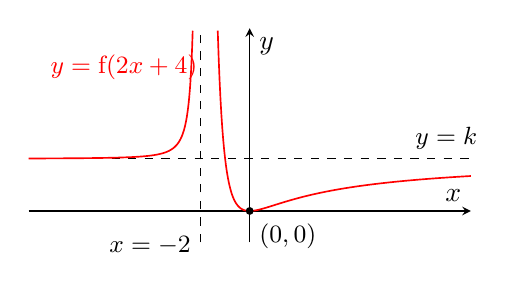
\begin{tikzpicture}
\begin{axis}[width=7.2cm,height=4.3cm,axis lines=middle,xmin=-9,xmax=9,ymin=-1.2,ymax=7,ticks=none,clip=false,restrict y to domain=-1.2:7,unbounded coords=jump,xlabel=$x$,ylabel=$y$]
\addplot[black,dashed,domain=-9:9]{2};
\addplot[black,dashed] coordinates{(-2,-1.2)(-2,7)};
\addplot[red,semithick,domain=-9:-2.04,samples=300]{2+0.5/(x+2)^2};
\addplot[red,semithick,domain=-1.96:9,samples=300]{2*(1-2/(x+2))^2};
\addplot[black,only marks,mark=*,mark size=1.2pt] coordinates{(0,0)};
\node[font=\small,anchor=north west] at (axis cs:0,-0.1){$(0,0)$};
\node[font=\small,anchor=south] at (axis cs:8,2){$y=k$};
\node[font=\small,anchor=north east] at (axis cs:-2,-0.6){$x=-2$};
\node[font=\small,red,anchor=west] at (axis cs:-8.5,5.5){$y=\mathrm{f}(2x+4)$};
\end{axis}\end{tikzpicture}\end{center}\end{gtpart}
\begin{gtpart}{(b)}{3}\begin{center}\begin{tikzpicture}
\begin{axis}[width=7.2cm,height=4.3cm,axis lines=middle,xmin=-7,xmax=10,ymin=-0.6,ymax=3.5,ticks=none,clip=false,restrict y to domain=-0.6:3.5,unbounded coords=jump,xlabel=$x$,ylabel=$y$]
\addplot[black,dashed,domain=-7:10]{0.5};
\addplot[black,dashed] coordinates{(2,-0.6)(2,3.5)};
\addplot[red,semithick,domain=-7:0,samples=300]{x^2/(2*x^2+0.5)};
\addplot[red,semithick,domain=0:1.97,samples=300]{x^2/(2*(x-2)^2)};
\addplot[red,semithick,domain=2.03:10,samples=300]{x^2/(2*(x-2)^2)};
\addplot[black,only marks,mark=*,mark size=1.2pt] coordinates{(0,0)};
\node[font=\small,anchor=north east] at (axis cs:0,0){$(0,0)$};
\node[font=\small,anchor=south] at (axis cs:-5.5,0.5){$y=\frac1k$};
\node[font=\small,anchor=north west] at (axis cs:2,-0.2){$x=2$};
\node[font=\small,red,anchor=west] at (axis cs:3.2,2.8){$y=\dfrac{1}{\mathrm{f}(2x)}$};
\end{axis}\end{tikzpicture}\end{center}\end{gtpart}
\begin{gtpart}{(c)}{3}\begin{center}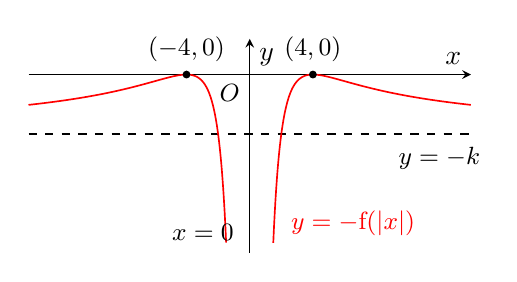
\begin{tikzpicture}
\begin{axis}[width=7.2cm,height=4.3cm,axis lines=middle,xmin=-14,xmax=14,ymin=-6,ymax=1.2,ticks=none,clip=false,restrict y to domain=-6:1.2,unbounded coords=jump,xlabel=$x$,ylabel=$y$]
\addplot[black,dashed,domain=-14:14]{-2};
\addplot[red,semithick,domain=0.3:14,samples=300]{-2*(1-4/x)^2};
\addplot[red,semithick,domain=-14:-0.3,samples=300]{-2*(1+4/x)^2};
\addplot[black,only marks,mark=*,mark size=1.2pt] coordinates{(4,0)(-4,0)};
\node[font=\small,anchor=south] at (axis cs:4,0.1){$(4,0)$};
\node[font=\small,anchor=south] at (axis cs:-4,0.1){$(-4,0)$};
\node[font=\small,anchor=north east] at (axis cs:0,0){$O$};
\node[font=\small,anchor=north] at (axis cs:12,-2.1){$y=-k$};
\node[font=\small,anchor=east] at (axis cs:-0.4,-5.3){$x=0$};
\node[font=\small,red,anchor=west] at (axis cs:2,-5){$y=-\mathrm{f}(|x|)$};
\end{axis}\end{tikzpicture}\end{center}\end{gtpart}}
%% ============================================================ 43  CJC 2025 Promo Q8
\defQ{43}{}{%
\mbox{}\par\vspace{-1ex}\begin{center}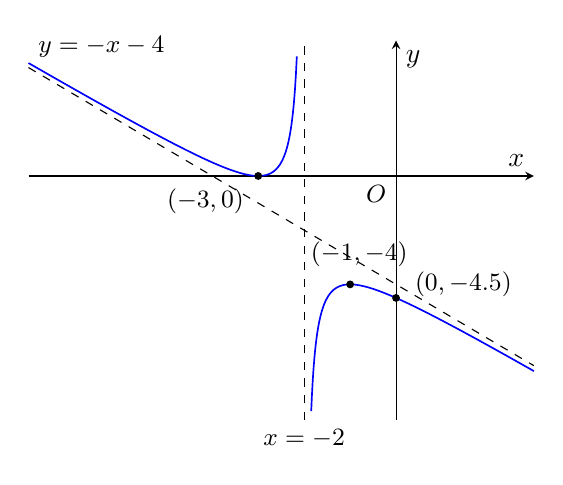
\begin{tikzpicture}
\begin{axis}[width=8cm,height=6.4cm,axis lines=middle,xmin=-8,xmax=3,ymin=-9,ymax=5,ticks=none,clip=false,restrict y to domain=-9:5,unbounded coords=jump,xlabel=$x$,ylabel=$y$]
\addplot[black,dashed] coordinates{(-2,-9)(-2,5)};
\addplot[black,dashed,domain=-8:3]{-x-4};
\addplot[blue,semithick,domain=-8:-2.02,samples=300]{-x-4-1/(x+2)};
\addplot[blue,semithick,domain=-1.98:3,samples=300]{-x-4-1/(x+2)};
\addplot[black,only marks,mark=*,mark size=1.2pt] coordinates{(-3,0)(-1,-4)(0,-4.5)};
\node[font=\small,anchor=north east] at (axis cs:0,0){$O$};
\node[font=\small,anchor=north east] at (axis cs:-3.1,-0.1){$(-3,0)$};
\node[font=\small,anchor=south] at (axis cs:-0.8,-3.7){$(-1,-4)$};
\node[font=\small,anchor=west] at (axis cs:0.2,-4){$(0,-4.5)$};
\node[font=\small,anchor=north] at (axis cs:-2,-9){$x=-2$};
\node[font=\small,anchor=south west] at (axis cs:-8,4){$y=-x-4$};
\end{axis}\end{tikzpicture}\end{center}
The diagram shows the curve $y=\mathrm{f}(x)$. The curve crosses the $x$-axis at its minimum point $(-3,0)$. It has a maximum turning point $(-1,-4)$ and crosses the $y$-axis at the point $(0,-4.5)$. The asymptotes of the curve are $x=-2$ and $y=-x-4$.\par
On separate diagrams, sketch the graphs of
\begin{qparts}
\pt{(a)} $y=\mathrm{f}'(x)$, \mk{3}
\pt{(b)} $y=\dfrac{1}{\mathrm{f}(x)}$, \mk{3}
\pt{(c)} $y=|\mathrm{f}(x)|$, \mk{3}
\end{qparts}
indicating the equations of any asymptotes, turning points and intersections with the axes.
\src{CJC 2025 Promo Q8}}
\defS{43}{%
\begin{gtpartn}{(a)}\begin{center}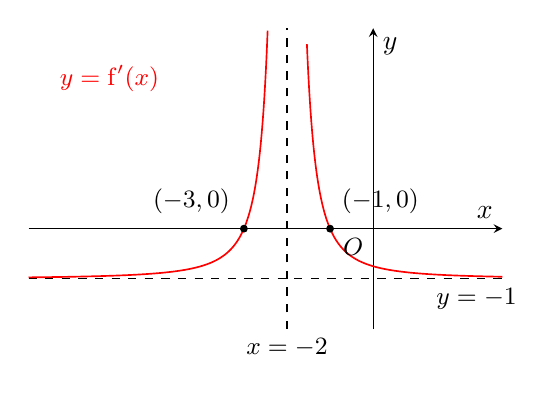
\begin{tikzpicture}
\begin{axis}[width=7.6cm,height=5.4cm,axis lines=middle,xmin=-8,xmax=3,ymin=-2,ymax=4,ticks=none,clip=false,restrict y to domain=-2:4,unbounded coords=jump,xlabel=$x$,ylabel=$y$]
\addplot[black,dashed] coordinates{(-2,-2)(-2,4)};
\addplot[black,dashed,domain=-8:3]{-1};
\addplot[red,semithick,domain=-8:-2.03,samples=300]{-1+1/(x+2)^2};
\addplot[red,semithick,domain=-1.97:3,samples=300]{-1+1/(x+2)^2};
\addplot[black,only marks,mark=*,mark size=1.2pt] coordinates{(-3,0)(-1,0)};
\node[font=\small,anchor=south east] at (axis cs:-3.1,0.1){$(-3,0)$};
\node[font=\small,anchor=south west] at (axis cs:-0.95,0.1){$(-1,0)$};
\node[font=\small,anchor=north east] at (axis cs:0,0){$O$};
\node[font=\small,anchor=north] at (axis cs:2.4,-1){$y=-1$};
\node[font=\small,anchor=north] at (axis cs:-2,-2){$x=-2$};
\node[font=\small,red,anchor=west] at (axis cs:-7.5,3){$y=\mathrm{f}'(x)$};
\end{axis}\end{tikzpicture}\end{center}\end{gtpartn}
\begin{gtpartn}{(b)}\begin{center}\begin{tikzpicture}
\begin{axis}[width=7.6cm,height=5.4cm,axis lines=middle,xmin=-9,xmax=4,ymin=-0.8,ymax=3,ticks=none,clip=false,restrict y to domain=-0.8:3,unbounded coords=jump,xlabel=$x$,ylabel=$y$]
\addplot[black,dashed] coordinates{(-3,-0.8)(-3,3)};
\addplot[red,semithick,domain=-9:-3.03,samples=300]{-(x+2)/(x+3)^2};
\addplot[red,semithick,domain=-2.97:4,samples=300]{-(x+2)/(x+3)^2};
\addplot[black,only marks,mark=*,mark size=1.2pt] coordinates{(-2,0)(-1,-0.25)(0,-0.2222)};
\node[font=\small,anchor=south west] at (axis cs:-1.9,0.05){$(-2,0)$};
\node[font=\small,anchor=north east] at (axis cs:-1.3,-0.3){$\left(-1,-\frac14\right)$};
\node[font=\small,anchor=north west] at (axis cs:0.3,-0.3){$\left(0,-\frac29\right)$};
\node[font=\small,anchor=north east] at (axis cs:0,0){$O$};
\node[font=\small,anchor=south] at (axis cs:-3,3){$x=-3$};
\node[font=\small,anchor=south] at (axis cs:-8,0.05){$y=0$};
\node[font=\small,red,anchor=west] at (axis cs:0.5,2){$y=\dfrac{1}{\mathrm{f}(x)}$};
\end{axis}\end{tikzpicture}\end{center}\end{gtpartn}
\begin{gtpartn}{(c)}\begin{center}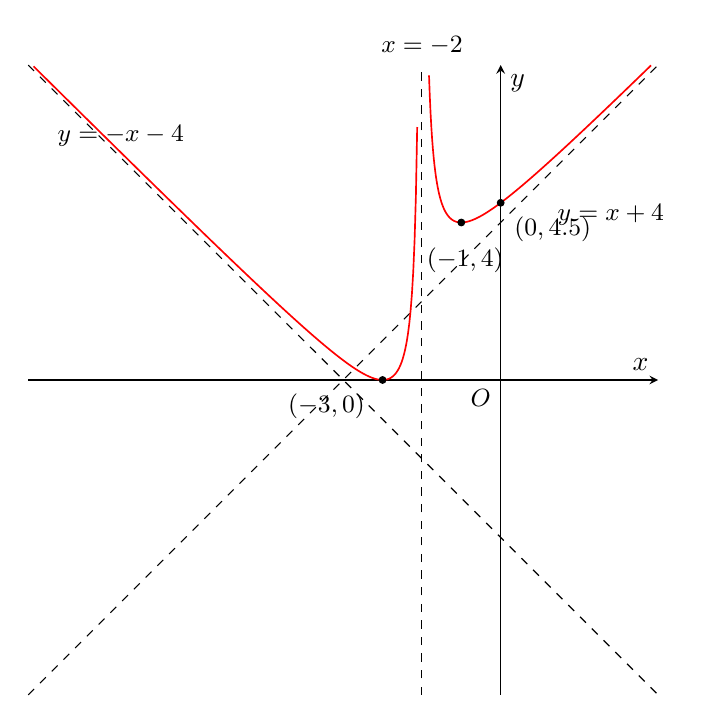
\begin{tikzpicture}
\begin{axis}[width=8cm,height=8cm,scale only axis,axis lines=middle,xmin=-12,xmax=4,ymin=-8,ymax=8,ticks=none,clip=false,restrict y to domain=-8:8,unbounded coords=jump,xlabel=$x$,ylabel=$y$]
\addplot[black,dashed] coordinates{(-2,-8)(-2,8)};
\addplot[black,dashed,domain=-12:4]{-x-4};
\addplot[black,dashed,domain=-12:4]{x+4};
\addplot[red,semithick,domain=-12:-2.02,samples=300]{abs(-x-4-1/(x+2))};
\addplot[red,semithick,domain=-1.98:4,samples=300]{abs(-x-4-1/(x+2))};
\addplot[black,only marks,mark=*,mark size=1.2pt] coordinates{(-3,0)(-1,4)(0,4.5)};
\node[font=\small,anchor=north east] at (axis cs:-3.2,-0.1){$(-3,0)$};
\node[font=\small,anchor=north] at (axis cs:-0.9,3.6){$(-1,4)$};
\node[font=\small,anchor=north west] at (axis cs:0.1,4.4){$(0,4.5)$};
\node[font=\small,anchor=north east] at (axis cs:0,0){$O$};
\node[font=\small,anchor=south] at (axis cs:-2,8){$x=-2$};
\node[font=\small,anchor=west] at (axis cs:-11.5,6.2){$y=-x-4$};
\node[font=\small,anchor=west] at (axis cs:1.2,4.2){$y=x+4$};
\end{axis}\end{tikzpicture}\end{center}\end{gtpartn}}
%% ============================================================ 44  RVHS 2026 Prelim P1 Q10(b)
\defQ{44}{}{%
Express $\dfrac{9x+5}{3x+2}$ in the form $a-\dfrac{b}{3x+2}$ where $a$ and $b$ are positive constants.\par
Hence, describe a sequence of transformations which transform the graph of $y=\dfrac{9x+5}{3x+2}$ to the graph of $y=\dfrac1x$. \mk{5}
\src{RVHS 2026 Prelim P1 Q10(b)}}
\defS{44}{%
\begin{gtpart}{(b)}{5}\begin{topalign}
\frac{9x+5}{3x+2}&=3-\frac{1}{3x+2}\qquad(a=3,\ b=1)\\
y=3-\frac{1}{3x+2}\ &\xrightarrow{\ y\to y+3\ }\ y=-\frac{1}{3x+2}\\
&\xrightarrow{\ y\to-y\ }\ y=\frac{1}{3x+2}\\
&\xrightarrow{\ x\to\frac x3\ }\ y=\frac{1}{x+2}\\
&\xrightarrow{\ x\to x-2\ }\ y=\frac1x
\end{topalign}
\begin{enumerate}\setlength\itemsep{0pt}
\item Translate 3 units in the negative $y$-direction
\item Reflect about the $x$-axis
\item Scale by factor 3 parallel to the $x$-axis
\item Translate 2 units in the positive $x$-direction
\end{enumerate}\end{gtpart}}
